\documentclass[11pt]{beamer}

\usetheme{Singapore}

\definecolor{DarkRed}{rgb}{0.50,0,0}
\definecolor{DarkGreen}{rgb}{0,0.50,0}
\definecolor{DarkBlue}{rgb}{0,0,0.50}
\definecolor{Black}{rgb}{0,0,0}

\newcommand{\ttdr}[1]{{\tt{\color{DarkRed} #1}}}
\newcommand{\emdr}[1]{{\em{\color{DarkRed} #1}}}
\newcommand{\ttdg}[1]{{\tt{\color{DarkGreen} #1}}}
\newcommand{\emdg}[1]{{\em{\color{DarkGreen} #1}}}
\newcommand{\ttdb}[1]{{\tt{\color{DarkBlue} #1}}}
\newcommand{\emdb}[1]{{\em{\color{DarkBlue} #1}}}

\setbeamertemplate{frametitle}{
\begin{centering}
{\Large \textbf{\textmd{\insertframetitle}}}
\end{centering}
}

\setbeamertemplate{navigation symbols}{}

\setbeamertemplate{footline}{%
\begin{center}
{\color{DarkBlue}{\large 
\insertframenumber}
\hspace{240pt}

\includegraphics[height=50pt]{png/PDBP.png}}
\end{center}
}

\begin{document}

\begin{frame}
\vspace{25pt}
\begin{center}
\LARGE{
\vspace{10pt}
{\color{DarkGreen}{
PDBP}}} \\
\end{center}
\vspace{10pt}
\begin{center}
\LARGE{
{\color{DarkRed}{
Program Description Based Programming \\
Scala eXchange}}}
\end{center}
\vspace{10pt}
\begin{center}
\LARGE{
{\color{DarkBlue}{
Luc Duponcheel}}}
\end{center}
\vspace{10pt}
\begin{center}
\LARGE{
{\color{DarkGreen}{
\today}}}
\end{center}
\end{frame}

\begin{frame}[fragile]
\frametitle{\begin{center}Intro\end{center}}
\begin{itemize}
\item<2-> this talk is about
\begin{itemize}
\item<3-> a \ttdg{Dotty} \emdb{library} \ttdg{PDBP}
\item<4-> inspired by the \emdb{ function-level programming language} \ttdg{FP}
\end{itemize}
\end{itemize}
\end{frame}

\begin{frame}[fragile]
\frametitle{\begin{center}John Backus\end{center}}
\begin{center}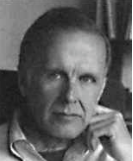
\includegraphics[height=60pt]{png/Backus.png}\end{center}
\begin{itemize}
\item<2-> ACM Turing Award Winner 1977
\item<3-> \emdb{Can programming be liberated from the Von Neumann style?}
\end{itemize}
\end{frame}

\begin{frame}[fragile]
\frametitle{\begin{center}What is this?\end{center}}
\begin{center}
\includegraphics[height=120pt]{png/PipeQuestion.png}\end{center}
\begin{itemize}
\item<2-> A \emdb{pipe}?
\item<3-> A \emdb{painting} \emdb{describing} a pipe?
\item<4-> A \emdb{slide} \emdb{describing} a painting describing a pipe?
\item<5-> \ldots
\end{itemize}
\end{frame}

\begin{frame}[fragile]
\frametitle{\begin{center}Ceci n'est pas une pipe\end{center}}
\begin{center}
\includegraphics[height=140pt]{png/Pipe.png}\end{center}
\begin{itemize}
\item<2-> It is a \emdb{painting} by Ren\'{e} Magritte \emdb{describing} a pipe
\end{itemize}
\end{frame}

\begin{frame}[fragile]
\frametitle{\begin{center}This is not a program\end{center}}
{\color{DarkGreen}	
\footnotesize{
\begin{verbatim}
  val xxxxxxxxx: BigInt >--> BigInt =
    `if`(isZero) {
      one
    } `else` {
      `let` {
        subtractOne >-->
          xxxxxxxxx
      } `in` {
        multiply
      }
    }
\end{verbatim}
}
}
\begin{center}
\begin{itemize}
\item<2-> It is \emdb{code} \emdb{describing} a program
\end{itemize}
\end{center}
\end{frame}

\begin{frame}[fragile]
\frametitle{\begin{center}\ttdg{factorial} description\end{center}}
{\color{DarkGreen}	
\footnotesize{
\begin{verbatim}
  val factorial: BigInt >--> BigInt =
    `if`(isZero) {
      one
    } `else` {
      `let` {
        subtractOne >-->
          factorial
      } `in` {
        multiply
      }
    }
\end{verbatim}
}
}
\begin{center}
\begin{itemize}
\item<2-> \ttdg{factorial} \emdb{uses} capabilities \emdb{declared} in \\ type class \ttdg{trait Program[>-->[- \_, + \_]]}
\end{itemize}
\end{center}
\end{frame}

\begin{frame}[fragile]
\frametitle{\begin{center}\ttdg{factorial} meanings\end{center}}
{\color{DarkGreen}	
\footnotesize{
\begin{verbatim}
  val factorial: BigInt >--> BigInt =
    `if`(isZero) {
      one
    } `else` {
      `let` {
        subtractOne >-->
          factorial
      } `in` {
        multiply
      }
    }
\end{verbatim}
}
}
\begin{center}
\begin{itemize}
\item<2-> different \ttdg{implicit object}'s \emdb{define} capabilities of \\ type class \ttdg{trait Program[>-->[- \_, + \_]]}
\end{itemize}
\end{center}
\end{frame}

\begin{frame}[fragile]
\frametitle{\begin{center}\ttdg{program}\end{center}}
{\color{DarkGreen}	
\begin{verbatim}
  val program: Z >--> Y
\end{verbatim}
}
\end{frame}

\begin{frame}[fragile]
\frametitle{\begin{center}Composition\end{center}}
{\color{DarkGreen}	
\begin{verbatim}
  val `z>-->y`: Z >--> Y
  val `y>-->x`: Y >--> x

  val `z>-->x`: Z >--> X =  `z>-->y >--> `y>-->x`
\end{verbatim}
}
\end{frame}

\begin{frame}[fragile]
\frametitle{\begin{center}\ttdg{mainProgram}\end{center}}
{\color{DarkGreen}	
\begin{verbatim}
  val producer: Unit >--> Z
  val program: Z >--> Y
  val consumer: Y >--> Unit

  val mainProgram: Unit >--> Unit =
    producer >--> program >--> consumer
\end{verbatim}
}
\end{frame}

\begin{frame}[fragile]
\frametitle{\begin{center}\ttdg{FP} versus \ttdg{PDBP}\end{center}}
\begin{itemize}
\item<2-> \ttdg{FP} and \ttdg{PDBP} promote \emdb{pointfree functional programming}
\item<3-> \ttdg{FP} is a \emdb{language} \\
\ttdg{PDBP} is a \emdb{library}
\begin{itemize}
\item<4-> \ttdg{FP} \emdb{semantics} is \emdb{fixed} \\ 
\ttdg{PDBP} \emdb{semantics} is \emdb{not fixed}
\item<5-> \ttdg{FP} \emdb{capabilities} are \emdb{fixed} \\ 
\ttdg{PDBP} \emdb{capabilities} are \emdb{not fixed}
\item<6-> \ttdg{FP} \emdb{effects} are \emdb{impure} \\ 
\ttdg{PDBP} \emdb{effects} are \emdb{pure}
\end{itemize}
\end{itemize}
\end{frame}

\begin{frame}[fragile]
\frametitle{\begin{center}Semantics\end{center}}
{\color{DarkGreen}	
\footnotesize{
\begin{verbatim}
  val factorial: BigInt >--> BigInt =
    `if`(isZero) {
      one
    } `else` {
      `let` {
        subtractOne >-->
          factorial
      } `in` {
        multiply
      }
    }
\end{verbatim}
}
}
\begin{itemize}
\item<2-> \emdb{production} 
\begin{itemize}
\item<3-> \emdb{recursion} using \emdb{stack} 
\item<4-> \emdb{recursion} using \emdb{heap}
\end{itemize}
\item<5-> \emdb{test}
\begin{itemize}
\item<6-> \ldots
\end{itemize}
\end{itemize}
\end{frame}

\begin{frame}[fragile]
\frametitle{\begin{center}Capabilities\end{center}}
\begin{itemize}
\item<2-> \emdb{manipulating state}
\item<3-> \emdb{handling failure}
\item<4-> \emdb{handling latency}
\item<5-> \emdb{handling control}
\item<6-> \emdb{\ldots}
\end{itemize}
\end{frame}

\begin{frame}[fragile]
\frametitle{\begin{center}Effects\end{center}}
\begin{itemize}
\item<2-> \emdb{reading} 
\item<3-> \emdb{writing}
\end{itemize}
\end{frame}

\begin{frame}[fragile]
\frametitle{\begin{center}Foundations\end{center}}
\begin{itemize}
\item<2-> \ttdg{trait Program[>-->[- \_, + \_]]} corresponds to \emdb{arrows}
\item<3-> \ttdg{trait Computation[C[+ \_]]} corresponds to \emdb{monads}
\end{itemize}
\end{frame}

\begin{frame}[fragile]
\frametitle{\begin{center}Monads versus arrows\end{center}}
\begin{itemize}
\item<2-> \emdb{arrows} (\ttdg{trait Program[>-->[- \_, + \_]]}) \\ generalize \emdb{functions}
\begin{itemize}
\item<3-> \emdb{composition} based, \emdb{pointfree} functional programming
\item<4-> \ttdg{val `z=>x` = `z=>y` andThen `y=>x`}
\item<5-> \ttdg{val `z>-->x` = `z>-->y` >--> `y>-->z`}
\end{itemize}
\item<6-> \emdb{monads} (\ttdg{trait Computation[C[+ \_]]}) \\ generalize \emdb{expressions} 
\begin{itemize}
\item<7-> \emdb{binding} based, \emdb{pointful} functional programming
\item<8-> \ttdg{\{ val z = ez ; \{ val y = ey ; ex(z, y) \} \} }
\item<9-> \ttdg{mz bind \{ z => my bind \{ y => mx(z, y) \} \} }
\item<10-> \ttdg{mz bind \{ z => my bind \{ y => result(ex(z, y)) \} \} }
\end{itemize}
\end{itemize}
\end{frame}

\begin{frame}[fragile]
\frametitle{\begin{center}Monads versus arrows\end{center}}
\begin{itemize}
\item<2-> \emdb{monads} can also be programmed \emdb{pointfree} (\emdb{kleisli arrows}) 
\item<3-> \emdb{arrows} can also be programmed \emdb{pointful} (\emdb{arrow calculus})
\end{itemize}
\end{frame}

\begin{frame}[fragile]
\frametitle{\begin{center}Power of expressions\end{center}}
\begin{itemize}
\item<2-> \emdb{monads} are more \emdb{concrete} (less \emdb{abstract}) than \emdb{arrows}
\begin{itemize}
\item<3-> \emdb{monads} allow more \emdb{specification liberty}
\item<4-> \emdb{monads} impose more \emdb{implementation constraints}
\end{itemize}
\item<5-> \emdb{Constraints Liberate, Liberties Constrain}
\end{itemize}
\end{frame}

\begin{frame}[fragile]
\frametitle{\begin{center}Elegance of use\end{center}}
\begin{itemize}
\item<2-> \emdb{pointfree} programming is sometimes considered to be more \emdb{abstruse} than \emdb{pointful} programming
\item<3-> \ttdg{Dotty} comes to the rescue
\begin{itemize}
\item<4-> \ttdg{Dotty} is a \ttdg{Sca}lable \ttdg{la}nguage
\item<5-> \ttdg{Dotty} \emdb{library based} language extensions are \emdb{type safe}
\end{itemize}
\item<6-> \ttdg{PDBP} comes with a \emdb{program description DSL}
\end{itemize}
\end{frame}

\begin{frame}[fragile]
\frametitle{\begin{center}Program description DSL\end{center}}
{\color{DarkGreen}	
\footnotesize{
\begin{verbatim}
  val factorial: BigInt >--> BigInt =
    `if`(isZero) {
      one
    } `else` {
      `let` {
        subtractOne >-->
          factorial
      } `in` {
        multiply
      }
    }
\end{verbatim}
}
}
\end{frame}

\begin{frame}[fragile]
\frametitle{\begin{center}\ttdg{PDBP}'s choice\end{center}}
\begin{itemize}
\item<2-> the \ttdg{PDBP} libary goes for
\begin{itemize}
\item<3-> \ttdg{private[pdbp]} \emdb{pointful monad API} \\
provides \emdb{power of expression} for \emdb{library} developers 
\item<4-> \ttdg{public} \emdb{pointfree arrow API} \\
provides \emdb{elegance of use} for \emdb{application} developers
\end{itemize}
\item<5->the \ttdg{PDBP} can live with
\begin{itemize}
\item<6-> corresponding implementation constraints
\end{itemize}
\end{itemize}
\end{frame}

\begin{frame}[fragile]
\frametitle{\begin{center}PDBP\end{center}}
{\color{DarkGreen}
\footnotesize{
\begin{verbatim}
  //       _______         __    __        _______
  //      / ___  /\       / /\  / /\      / ___  /\
  //     / /__/ / / _____/ / / / /_/__   / /__/ / /
  //    / _____/ / / ___  / / / ___  /\ /____  / /
  //   / /\____\/ / /__/ / / / /__/ / / \___/ / /
  //  /_/ /      /______/ / /______/ /     /_/ /
  //  \_\/       \______\/  \______\/      \_\/
  //                                           v1.0
  //  Program Description Based Programming Library
  //  author        Luc Duponcheel        2017-2018 
\end{verbatim}
}
}
\end{frame}

\begin{frame}[fragile]
\frametitle{\begin{center}\ttdg{PDBP} library design decisions (cfr. \ttdg{Haskell})\end{center}}
\begin{itemize}
\item<2-> \emdb{description} separated from \emdb{meaning}
\item<3-> \emdb{description}
\begin{itemize}
\item<4-> \ttdg{trait}'s (\emdb{type classes}) \emdb{declare} capabilities 
\end{itemize}
\item<5-> \emdb{language level} meaning
\begin{itemize}
\item<6-> \ttdg{implicit object}'s (\ttdg{extend} \ttdg{trait}'s) \emdb{define} capabilities 
\end{itemize}
\item<7-> \emdb{library level} meaning
\begin{itemize}
\item<8-> \emdb{natural transformations}
\end{itemize}
\end{itemize}
\end{frame}

\begin{frame}[fragile]
\frametitle{\begin{center}\ttdg{PDBP} library design decisions (cfr. \ttdg{Haskell})\end{center}}
\begin{itemize}
\item<2-> \emdb{dependency injection} by \ttdg{implicit import}
\end{itemize}
\begin{itemize}
\item<3-> \emdb{definitions} in \ttdg{class}'es that \emdb{implicitly} depend on \ttdg{trait}'s (\emdb{type classes})
use capabilities \emdb{declared} in those \ttdg{trait}'s
\item<4-> \ttdg{object}'s that \emdb{extend} those \ttdg{class}'es \ttdg{import} \ttdg{implicit object}'s that \emdb{extend} those \ttdg{trait}'s
\end{itemize}
\end{frame}

\begin{frame}[fragile]
\frametitle{\begin{center}\ttdg{Program} (cfr. \emdb{arrow})\end{center}}
{\color{DarkGreen}	
\footnotesize{
\begin{verbatim}
  trait Program[>-->[- _, + _]]
\end{verbatim}
}
}
\end{frame}

\begin{frame}[fragile]
\frametitle{\begin{center}\ttdg{Computation} (cfr. \emdb{monad})\end{center}}
{\color{DarkGreen}	
\footnotesize{
\begin{verbatim}
  trait Computation[C[+ _]]
\end{verbatim}
}
}
\end{frame}

\begin{frame}[fragile]
\frametitle{\begin{center}Liskov Substitution Principle\end{center}}
\begin{itemize}
\item<2-> \emdb{impose less}
\item<3-> \emdb{provide more}
\end{itemize}
\end{frame}

\begin{frame}[fragile]
\frametitle{\begin{center}Internet Robustness Principle\end{center}}
\begin{itemize}
\item<2-> \emdb{be liberal in what you receive}
\item<3-> \emdb{be generous in what you send}
\end{itemize}
\end{frame}

\begin{frame}[fragile]
\frametitle{\begin{center}\ttdg{PDBP} library details\end{center}}
\end{frame}

\begin{frame}[fragile]
\frametitle{\begin{center}\ttdg{Program}\end{center}}
{\color{DarkGreen}	
\footnotesize{
\begin{verbatim}
  trait Program[>-->[- _, + _]]
      extends Function[>-->] 
      with Composition[>-->] 
      with Construction[>-->] 
      with Condition[>-->]

      with Aggregation[>-->] 
\end{verbatim}
}
}
\end{frame}

\begin{frame}[fragile]
\frametitle{\begin{center}\ttdg{Function}\end{center}}
\begin{itemize}	
\item<2->
{\color{DarkGreen}	
\footnotesize{
\begin{verbatim}
      val `z>-->y` = function(`z=>y`) 
\end{verbatim}
}
}
\item<3-> pure functions are \emdb{atomic programs}
\begin{itemize}	
\item<4-> up to you to define granularity
\end{itemize}
\end{itemize}
\end{frame}

\begin{frame}[fragile]
\frametitle{\begin{center}\ttdg{Composition}\end{center}}
\begin{itemize}	
\item<2->
{\color{DarkGreen}
\footnotesize{
\begin{verbatim}
      val `z>-->x` = `z>-->y` >--> `y>-->x`
\end{verbatim}
}
}
\end{itemize}
\end{frame}

\begin{frame}[fragile]
\frametitle{\begin{center}\ttdg{Construction}\end{center}}
\begin{itemize}	
\item<2->
{\color{DarkGreen}
\footnotesize{
\begin{verbatim}
      val `z>-->y&&x` = `z>-->y` & `z>-->x`
\end{verbatim}
}
}
\item<3->
{\color{DarkGreen}
\footnotesize{
\begin{verbatim}
      val `z&&y>-->x&&w` = `z>-->x` && `y>-->w`
\end{verbatim}
}
}
\item<4->
{\color{DarkGreen}
\footnotesize{
\begin{verbatim}
      val `z>-->x` = 
         `let` `z>-->y` `in` `z&&y>-->x`
\end{verbatim}
}
}
\end{itemize}
\end{frame}

\begin{frame}[fragile]
\frametitle{\begin{center}\ttdg{Condition}\end{center}}
\begin{itemize}	
\item<2->
{\color{DarkGreen}
\footnotesize{
\begin{verbatim}
      val `y||x>-->z` = `y>-->z` | `x>-->z`
\end{verbatim}
}
}
\item<3->
{\color{DarkGreen}
\footnotesize{
\begin{verbatim}
      val `x||w>-->z||y` = `x>-->z` || `w>-->y`
\end{verbatim}
}
}
\item<4->
{\color{DarkGreen}
\footnotesize{
\begin{verbatim}
      val `y>-->z` = 
          `if`(`y>-->b`) `y>-t->z` `else` `y>-f->z`
\end{verbatim}
}
}
\end{itemize}
\end{frame}

\begin{frame}[fragile]
\frametitle{\begin{center}\ttdg{Computation}\end{center}}
{\color{DarkGreen}	
\footnotesize{
\begin{verbatim}
  private[pdbp] trait Computation[C[+ _]]
      extends Resulting[C] 
      with Binding[C] 
      with Program[[-Z, +Y] => Z => C[Y]]

      with Lifting[C]

      with Sequencing[C]

\end{verbatim}
}
}
\end{frame}

\begin{frame}[fragile]
\frametitle{\begin{center}\ttdg{Resulting}\end{center}}
{\color{DarkGreen}	
\footnotesize{
\begin{verbatim}
  val cz = result(z)
\end{verbatim}
}
}
\end{frame}

\begin{frame}[fragile]
\frametitle{\begin{center}\ttdg{Binding}\end{center}}
\begin{itemize}	
\item<2-> 
{\color{DarkGreen}
\footnotesize{
\begin{verbatim}
  val cy = cz bind { z => `z=>cy`(y) }

\end{verbatim}
}
}
\item<3->
{\color{DarkGreen}
\footnotesize{
\begin{verbatim}
  val cy = cz bind { z => result(`z=>y`(y)) }
\end{verbatim}
}
}
\end{itemize}
\end{frame}

\begin{frame}[fragile]
\frametitle{\begin{center}\ttdg{Kleisli}\end{center}}
\begin{itemize}	
\item<2-> 
{\color{DarkGreen}
\footnotesize{
\begin{verbatim}
  type Kleisli[C[+ _]] = [-Z, + Y] => Z => C[Y]

\end{verbatim}
}
}
\item<3->
{\color{DarkGreen}
\footnotesize{
\begin{verbatim}
  private[pdbp] trait Computation[C[+ _]]
      extends Resulting[C] 
      with Binding[C] 
      with Program[Kleisli[C]]

      // ...
\end{verbatim}
}
}
\end{itemize}
\end{frame}

\begin{frame}[fragile]
\frametitle{\begin{center}\ttdg{HelperFunctions}\end{center}}
{\color{DarkGreen}	
\footnotesize{
\begin{verbatim}
  val isZeroFunction: BigInt => Boolean = 
  { i =>
      i == 0
  }
  def oneFunction[Z]: Z => BigInt = 
  { z =>
      1
  }
  val subtractOneFunction: BigInt => BigInt = 
  { i =>
      i - 1
  }
  val multiplyFunction: (BigInt && BigInt) => BigInt = 
  { (i, j) =>
      i * j
  }
\end{verbatim}
}
}
\end{frame}

\begin{frame}[fragile]
\frametitle{\begin{center}\ttdg{HelperPrograms}\end{center}}
{\color{DarkGreen}	
\footnotesize{
\begin{verbatim}
  val isZeroHelper: BigInt >--> Boolean =
    function(isZeroFunction)

  val subtractOneHelper: BigInt >--> BigInt =
    function(subtractOneFunction)

  val multiplyHelper: (BigInt && BigInt) >--> BigInt =
    function(multiplyFunction)

  def oneHelper[Z]: Z >--> BigInt =
    function(oneFunction)
\end{verbatim}
}
}
\end{frame}

\begin{frame}[fragile]
\frametitle{\begin{center}\ttdg{AtomicPrograms}\end{center}}
{\color{DarkGreen}	
\footnotesize{
\begin{verbatim}
  val isZero: BigInt >--> Boolean =
    isZeroHelper

  val subtractOne: BigInt >--> BigInt =
    subtractOneHelper

  val multiply: (BigInt && BigInt) >--> BigInt =
    multiplyHelper

  def one[Z]: Z >--> BigInt =
    oneHelper
\end{verbatim}
}
}
\end{frame}

\begin{frame}[fragile]
\frametitle{\begin{center}\ttdg{factorial}\end{center}}
{\color{DarkGreen}	
\footnotesize{
\begin{verbatim}
  val factorial: BigInt >--> BigInt =
    `if`(isZero) {
      one
    } `else` {
      `let` {
        subtractOne >-->
          factorial
      } `in` {
        multiply
      }
    }
\end{verbatim}
}
}
\end{frame}

\begin{frame}[fragile]
\frametitle{\begin{center}\ttdg{factorialMain}\end{center}}
{\color{DarkGreen}	
\footnotesize{
\begin{verbatim}
  val factorialMain: Unit >--> Unit =
    producer >-->
      factorial >-->
      consumer
\end{verbatim}
}
}
\end{frame}

\begin{frame}[fragile]
\frametitle{\begin{center}\ttdg{activeTypes}\end{center}}
{\color{DarkGreen}	
\footnotesize{
\begin{verbatim}
  object activeTypes {

    type Active[+Z] = Z

    type `=>A` = Kleisli[Active]

  }
\end{verbatim}
}
}
\end{frame}

\begin{frame}[fragile]
\frametitle{\begin{center}\ttdg{activeProgram}\end{center}}
{\color{DarkGreen}	
\footnotesize{
\begin{verbatim}
  implicit object activeProgram
      extends Computation[Active]
      with Program[`=>A`] {

    override private[pdbp] def result[Z]: Z => Active[Z] = 
      `z=>az`

    override private[pdbp] def bind[Z, Y](
        az: Active[Z],
        `z=>ay`: => (Z => Active[Y])): Active[Y] = 
      `z=>ay`(az)  

  }
\end{verbatim}
}
}
\end{frame}

\begin{frame}[fragile]
\frametitle{\begin{center}\ttdg{Main}\end{center}}
{\color{DarkGreen}	
\footnotesize{
\begin{verbatim}
  trait Main[>-->[- _, + _]] {

    val mainKleisliProgram: Unit >--> Unit
 
    val run: Unit

    def main(args: Array[String]): Unit = {

      run

    }    

  }
\end{verbatim}
}
}
\end{frame}

\begin{frame}[fragile]
\frametitle{\begin{center}\ttdg{FactorialMain}\end{center}}
{\color{DarkGreen}	
\footnotesize{
\begin{verbatim}
  object FactorialMain extends Main[`=>A`] {

    override val mainKleisliProgram: Unit `=>A` Unit = 
      factorialMain
 
    override val run = 
      mainKleisliProgram(())

  }
\end{verbatim}
}
}
\end{frame}

\begin{frame}[fragile]
\frametitle{\begin{center}Problems and Solutions\end{center}}
\begin{itemize}
\item<2-> Problem: obvious \ttdg{factorial} meaning \\
implementing \ttdg{>-->} as \ttdg{`=>A`} \emdb{is not stack safe}
\begin{itemize}
\item<3-> Solution: \ttdg{FreeTransformation} and \ttdg{FreeTransformedMeaning}
\end{itemize}
\item<4-> Problem: obvious \ttdg{producer} and \ttdg{consumer} \emdb{execute effects}
\begin{itemize}
\item<5-> Solution: \ttdg{Reading} resp. \ttdg{Writing} extensions of \ttdg{Program}
with members \ttdg{read} resp. \ttdg{write} that \emdb{describe effects}
\end{itemize}
\end{itemize}
\end{frame}

\begin{frame}[fragile]
\frametitle{\begin{center}\ttdg{NaturalBinaryTypeConstructorTransformation}\end{center}}
{\color{DarkGreen}	
\footnotesize{
\begin{verbatim}
  trait `-B->`[`>-F->`[- _, + _], `>-T->`[- _, + _]] {

    def apply[Z, Y]: Z `>-F->` Y => Z `>-T->` Y

  }
\end{verbatim}
}
}
\end{frame}

\begin{frame}[fragile]
\frametitle{\begin{center}\ttdg{NaturalUnaryTypeConstructorTransformation}\end{center}}
{\color{DarkGreen}	
\footnotesize{
\begin{verbatim}
  private[pdbp] trait `-U->`[F[+ _], T[+ _]]
      extends `-B->`[Kleisli[F], Kleisli[T]] {

    private[pdbp] def apply[Z](fz: F[Z]): T[Z]

    // ...
    }

  }
\end{verbatim}
}
}
\end{frame}

\begin{frame}[fragile]
\frametitle{\begin{center}\ttdg{ComputationTransformation}\end{center}}
{\color{DarkGreen}	
\footnotesize{
\begin{verbatim}
  private[pdbp] trait ComputationTransformation[
      FC[+ _]: Computation, T[+ _]] {

    private[pdbp] val transform: FC `-U->` T

  }
\end{verbatim}
}
}
\end{frame}

\begin{frame}[fragile]
\frametitle{\begin{center}\ttdg{FreeTransformed}\end{center}}
{\color{DarkGreen}	
\footnotesize{
\begin{verbatim}
  sealed trait Free[C[+ _], +Z]

  final case class Transform[C[+ _], +Z]
    (cz: C[Z]) extends Free[C, Z]
  final case class Result[C[+ _], +Z]
    (z: Z) extends Free[C, Z]
  final case class Bind[C[+ _], -Z, ZZ <: Z, +Y]
    (fczz: Free[C, ZZ], `z=>fcy`: Z => Free[C, Y])
      extends Free[C, Y]

  type FreeTransformed[C[+ _]] = [+Z] => Free[C, Z]
\end{verbatim}
}
}
\end{frame}

\begin{frame}[fragile]
\frametitle{\begin{center}\ttdg{FreeTransformation}\end{center}}
{\color{DarkGreen}	
\footnotesize{
\begin{verbatim}
  private[pdbp] 
    trait FreeTransformation[C[+ _]: Computation]
      extends Computation[FreeTransformed[C]]
      with Program[Kleisli[FreeTransformed[C]]]
      with Transformation[C, FreeTransformed[C]] {

    // unfold
    // transform => Transform
    // result => Result
    // bind => Bind

  }
\end{verbatim}
}
}
\end{frame}

\begin{frame}[fragile]
\frametitle{\begin{center}\ttdg{activeFreeTypes}\end{center}}
{\color{DarkGreen}	
\footnotesize{
\begin{verbatim}
  object activeFreeTypes {

    type ActiveFree = FreeTransformed[Active]

    type `=>AF` = Kleisli[ActiveFree]

  }
\end{verbatim}
}
}
\end{frame}

\begin{frame}[fragile]
\frametitle{\begin{center}\ttdg{activeFreeProgram}\end{center}}
{\color{DarkGreen}	
\footnotesize{
\begin{verbatim}
  import ... activeProgram

  implicit object activeFreeProgram
      extends Computation[ActiveFree]
      with Program[`=>AF`]
      with FreeTransformation[Active]()
      with ComputationTransformation[Active, ActiveFree]()
\end{verbatim}
}
}
\end{frame}

\begin{frame}[fragile]
\frametitle{\begin{center}\ttdg{ProgramMeaning}\end{center}}
{\color{DarkGreen}	
\footnotesize{
\begin{verbatim}
  trait ProgramMeaning[
    `>-FP->`[- _, + _]: Program, `>-T->`[- _, + _]] {

    private[pdbp] lazy val binaryTransformation: 
        `>-FP->` `-B->` `>-T->`

    lazy val meaning: `>-FP->` `-B->` `>-T->` = 
      binaryTransformation

  }
\end{verbatim}
}
}
\end{frame}

\begin{frame}[fragile]
\frametitle{\begin{center}\ttdg{ComputationMeaning}\end{center}}
{\color{DarkGreen}	
\footnotesize{
\begin{verbatim}
  private[pdbp] trait ComputationMeaning[
    FC[+ _]: Computation, T[+ _]]
      extends ProgramMeaning[Kleisli[FC], Kleisli[T]] {

    private[pdbp] val unaryTransformation: FC `-U->` T

    // ...

  }
\end{verbatim}
}
}
\end{frame}

\begin{frame}[fragile]
\frametitle{\begin{center}\ttdg{FreeTransformedMeaning}\end{center}}
{\color{DarkGreen}	
\footnotesize{
\begin{verbatim}
  private[pdbp] trait FreeTransformedMeaning[
    FC[+ _]: Computation, T[+ _]](
    implicit toBeTransformedMeaning: ComputationMeaning[FC, T])
    extends ComputationMeaning[FreeTransformed[FC], T] {

    // tailrecFold
    // Transform(fcz) => fcz
    // Result(z) => result(z)
    // Bind(Result(y), y2ftfcz) => tailrecFold(y2ftfcz(y))
    // Bind(Bind(fcx, x2ftfcy), y2ftfcz) => 
    //   tailrecFold(Bind(fcx, Bind(x2ftfcy, y2ftfcz)))

  }       
\end{verbatim}
}
}
\end{frame}

\begin{frame}[fragile]
\frametitle{\begin{center}\ttdg{activeMeaningOfActiveFree}\end{center}}
{\color{DarkGreen}	
\footnotesize{
\begin{verbatim}
  implicit object activeMeaningOfActive
      extends MeaningOfActive[Active]()
      with ComputationMeaning[Active, Active]()
      with ProgramMeaning[`=>A`, `=>A`]()

  import ... activeMeaningOfActive

  implicit object activeMeaningOfActiveFree
      extends FreeTransformedMeaning[Active, Active]()
      with ComputationMeaning[ActiveFree, Active]()
      with ProgramMeaning[`=>AF`, `=>A`]()    
\end{verbatim}
}
}
\end{frame}

\begin{frame}[fragile]
\frametitle{\begin{center}\ttdg{FactorialMain}\end{center}}
{\color{DarkGreen}	
\footnotesize{
\begin{verbatim}
  import activeMeaningOfActiveFree.meaning
  import mainFactorial.factorialMain

  object FactorialMain extends Main[`=>A`] {

    override val mainKleisliProgram: Unit `=>A` Unit = 
      meaning(factorialMain)
 
    override val run = mainKleisliProgram(())

  }
\end{verbatim}
}
}
\end{frame}

\begin{frame}[fragile]
\frametitle{\begin{center}\ttdg{Reading}\end{center}}
{\color{DarkGreen}	
\footnotesize{
\begin{verbatim}
  trait Reading[R, >-->[- _, + _]] {
    this: Function[>-->] & Composition[>-->] =>

    private[pdbp] def `u>-->r`: Unit >--> R 






  }
\end{verbatim}
}
}
\end{frame}

\begin{frame}[fragile]
\frametitle{\begin{center}\ttdg{Reading}\end{center}}
{\color{DarkGreen}	
\footnotesize{
\begin{verbatim}
  trait Reading[R, >-->[- _, + _]] {
    this: Function[>-->] & Composition[>-->] =>

    private[pdbp] def `u>-->r`: Unit >--> R = 
      `z>-->r`[Unit]

    private[pdbp] def `z>-->r`[Z]: Z >--> R =
      compose(`z>-->u`, `u>-->r`)

    

  }
\end{verbatim}
}
}
\end{frame}

\begin{frame}[fragile]
\frametitle{\begin{center}\ttdg{Reading}\end{center}}
{\color{DarkGreen}	
\footnotesize{
\begin{verbatim}
  trait Reading[R, >-->[- _, + _]] {
    this: Function[>-->] & Composition[>-->] =>

    private[pdbp] def `u>-->r`: Unit >--> R = 
      `z>-->r`[Unit]

    private[pdbp] def `z>-->r`[Z]: Z >--> R =
      compose(`z>-->u`, `u>-->r`)

    def read[Z]: Z >--> R = `z>-->r`

  }
\end{verbatim}
}
}
\end{frame}

\begin{frame}[fragile]
\frametitle{\begin{center}\ttdg{ReadingTransformed}\end{center}}
{\color{DarkGreen}	
\footnotesize{
\begin{verbatim}
  type `I=>`[-X, +Y] = implicit X => Y

  type ReadingTransformed[R, C[+ _]] = [+Z] => R `I=>` C[Z]
\end{verbatim}
}
}
\end{frame}

\begin{frame}[fragile]
\frametitle{\begin{center}\ttdg{ReadingTransformation}\end{center}}
{\color{DarkGreen}	
\footnotesize{
\begin{verbatim}
  private[pdbp] trait ReadingTransformation[
    R, FC[+ _]: Computation]
      extends ComputationTransformation[
        FC, ReadingTransformed[R, FC]]
      with Computation[ReadingTransformed[R, FC]]
      with Program[Kleisli[ReadingTransformed[R, FC]]]
      with Reading[R, Kleisli[ReadingTransformed[R, FC]]] {

    // ...

  }      
\end{verbatim}
}
}
\end{frame}

\begin{frame}[fragile]
\frametitle{\begin{center}\ttdg{factorialMain}\end{center}}
{\color{DarkGreen}	
\footnotesize{
\begin{verbatim}
  val factorialMain: Unit >--> Unit =
    read >-->
      factorial >-->
      consumer
\end{verbatim}
}
}
\end{frame}

\begin{frame}[fragile]
\frametitle{\begin{center}\ttdg{activeReadingTypes}\end{center}}
{\color{DarkGreen}	
\footnotesize{
\begin{verbatim}
  object activeReadingTypes {

    type ActiveReading[R] = ReadingTransformed[R, Active]

    type `=>AR`[R] = Kleisli[ActiveReading[R]]

  }
\end{verbatim}
}
}
\end{frame}

\begin{frame}[fragile]
\frametitle{\begin{center}\ttdg{activeIntReadingProgram}\end{center}}
{\color{DarkGreen}	
\footnotesize{
\begin{verbatim}
  import  ... activeProgram

  implicit object activeIntReadingProgram
      extends ActiveReadingProgram[BigInt]()
      with Computation[ActiveReading[BigInt]]()
      with Program[`=>AR`[BigInt]]()
      with Reading[BigInt, `=>AR`[BigInt]]()      
      with ReadingTransformation[BigInt, Active]()
      with ComputationTransformation[Active, ActiveReading[BigInt]]()
\end{verbatim}
}
}
\end{frame}

\begin{frame}[fragile]
\frametitle{\begin{center}\ttdg{FactorialMain}\end{center}}
{\color{DarkGreen}	
\footnotesize{
\begin{verbatim}
  object FactorialOfIntReadMain extends Main[`=>AR`[BigInt]] {

    import ... readIntFromConsoleEffect

    private type `=>AR[BigInt]` = `=>AR`[BigInt]

    override val mainKleisliProgram: Unit `=>AR[BigInt]` Unit = 
      factorialMain
    
    override val run = 
      mainKleisliProgram(())

  }
\end{verbatim}
}
}
\end{frame}

\begin{frame}[fragile]
\frametitle{\begin{center}\ttdg{factorialMultipliedByIntRead}\end{center}}
{\color{DarkGreen}	
\footnotesize{
\begin{verbatim}
  val factorialMultipliedByIntRead: BigInt >--> BigInt =
      (factorial & read) >--> multiply 
\end{verbatim}
}
}
\end{frame}

\begin{frame}[fragile]
\frametitle{\begin{center}\ttdg{Writing}\end{center}}
{\color{DarkGreen}	
\footnotesize{
\begin{verbatim}
  trait Writing[W: Writable, >-->[- _, + _]] {
    this: Function[>-->] & Composition[>-->] =>

    private[pdbp] val `w>-->u`: W >--> Unit  




    // ...

  }
\end{verbatim}
}
}
\end{frame}

\begin{frame}[fragile]
\frametitle{\begin{center}\ttdg{Writing}\end{center}}
{\color{DarkGreen}	
\footnotesize{
\begin{verbatim}
  trait Writing[W: Writable, >-->[- _, + _]] {
    this: Function[>-->] & Composition[>-->] =>

    private[pdbp] val `w>-->u`: W >--> Unit 
      = write(identity)

    def write[Z]: (Z => W) `I=>` Z >--> Unit =
      compose(function(implicitly), `w>-->u`)

    // ...

  }
\end{verbatim}
}
}
\end{frame}

\begin{frame}[fragile]
\frametitle{\begin{center}\ttdg{Writing}\end{center}}
{\color{DarkGreen}	
\footnotesize{
\begin{verbatim}
  def writeUsing[Z, Y, X](
      `(z&&y)=>x`: ((Z && Y) => X)): 
      (Z >--> Y) => ((X => W) `I=>` Z >--> Y) = { `z>-->y` =>
      val `(z&&y)>-->x` = function(`(z&&y)=>x`)
      val `z>-->(x&&y)` =
        `let` {
          `z>-->y`
        } `in` {
          `let` {
            `(z&&y)>-->x`
          } `in` {
            `(z&&y&&x)>-->(x&&y)`
          }
        }
      compose(compose(`z>-->(x&&y)`, left(write)), 
        `(u&&y)>-->y`)
  }          
\end{verbatim}
}
}
\end{frame}

\begin{frame}[fragile]
\frametitle{\begin{center}\ttdg{Writable}\end{center}}
{\color{DarkGreen}	
\footnotesize{
\begin{verbatim}
  private[pdbp] trait Writable[W]
      extends Startable[W]
      with Appendable[W]
\end{verbatim}
}
}
\end{frame}

\begin{frame}[fragile]
\frametitle{\begin{center}\ttdg{Startable}\end{center}}
{\color{DarkGreen}	
\footnotesize{
\begin{verbatim}
  private[pdbp] trait Startable[W] {

    private[pdbp] val start: W

  }
\end{verbatim}
}
}
\end{frame}

\begin{frame}[fragile]
\frametitle{\begin{center}\ttdg{Appendable}\end{center}}
{\color{DarkGreen}	
\footnotesize{
\begin{verbatim}
  private[pdbp] trait Appendable[W] {

    private[pdbp] val append: W && W => W

  }
\end{verbatim}
}
}
\end{frame}

\begin{frame}[fragile]
\frametitle{\begin{center}\ttdg{WritingTransformed}\end{center}}
{\color{DarkGreen}	
\footnotesize{
\begin{verbatim}
  type WritingTransformed[W, FC[+ _]] = [+Z] => FC[W && Z]
\end{verbatim}
}
}
\end{frame}

\begin{frame}[fragile]
\frametitle{\begin{center}\ttdg{WritingTransformation}\end{center}}
{\color{DarkGreen}	
\footnotesize{
\begin{verbatim}
  private[pdbp] trait WritingTransformation[
    W: Writable, FC[+ _]: Computation]
      extends ComputationTransformation[
        FC, WritingTransformed[W, FC]]
      with Computation[WritingTransformed[W, FC]]
      with Program[Kleisli[WritingTransformed[W, FC]]]
      with Writing[W, Kleisli[WritingTransformed[W, FC]]] {

    // ...

  }      
\end{verbatim}
}
}
\end{frame}

\begin{frame}[fragile]
\frametitle{\begin{center}\ttdg{ToConsole}\end{center}}
{\color{DarkGreen}	
\footnotesize{
\begin{verbatim}
  case class ToConsole(effect: Effect)

  type Effect = Unit => Unit
\end{verbatim}
}
}
\end{frame}

\begin{frame}[fragile]
\frametitle{\begin{center}\ttdg{ToConsole}\end{center}}
{\color{DarkGreen}	
\footnotesize{
\begin{verbatim}
  implicit object toConsoleWritable extends Writable[ToConsole] {

    override private[pdbp] val start: ToConsole =
      ToConsole { _ =>
        ()
      }

    override private[pdbp] val append: 
        ToConsole && ToConsole => ToConsole = {
      (tc1, tc2) =>
        ToConsole { _ =>
          { tc1.effect(()); tc2.effect(()) }
        }
    }

  }
\end{verbatim}
}
}
\end{frame}

\begin{frame}[fragile]
\frametitle{\begin{center}\ttdg{factorialMain}\end{center}}
{\color{DarkGreen}	
\footnotesize{
\begin{verbatim}
  val factorialMain: 
      (String => ToConsole) `I=>` 
          ((BigInt => ToConsole) `I=>` Unit >--> Unit) =
    read >-->
      factorial >-->
      write
\end{verbatim}
}
}
\end{frame}

\begin{frame}[fragile]
\frametitle{\begin{center}\ttdg{activeIntReadingWithWritingToConsoleProgram}\end{center}}
{\color{DarkGreen}	
\footnotesize{
\begin{verbatim}
  import ... toConsoleWritable
  import ... activeWritingToConsoleProgram

  implicit object activeIntReadingWithWritingToConsoleProgram
      extends ActiveReadingWithWritingProgram[BigInt, ToConsole]()
      with Computation[ActiveReadingWithWriting[BigInt, ToConsole]]()
      with Program[`=>ARW`[BigInt, ToConsole]]()                                            
      with Reading[BigInt, `=>ARW`[BigInt, ToConsole]]()
      with Writing[ToConsole, `=>ARW`[BigInt, ToConsole]]()
      // ...
\end{verbatim}
}
}
\end{frame}

\begin{frame}[fragile]
\frametitle{\begin{center}\ttdg{activeIntReadingWithWritingToConsoleProgram}\end{center}}
{\color{DarkGreen}	
\footnotesize{
\begin{verbatim}
      // ...
      with ReadingWithWritingTransformation[BigInt,
                                            ToConsole,
                                            ActiveWriting[ToConsole]]()
      with ReadingTransformation[BigInt, ActiveWriting[ToConsole]]()
      with ComputationTransformation[
        ActiveWriting[ToConsole],
        ActiveReadingWithWriting[BigInt, ToConsole]]()
\end{verbatim}
}
}
\end{frame}
\begin{frame}[fragile]
\frametitle{\begin{center}\ttdg{infoUtils}\end{center}}
{\color{DarkGreen}	
\footnotesize{
\begin{verbatim}
  def infoFunction[Z, Y](string: String): Z && Y => String = {
    case (z, y) =>
      s"INFO -- $currentCalendarInMilliseconds -- $string($z) => $y"
  }

  def info[
      W: Writable, Z, Y,  
      >-->[- _, + _]: [>-->[- _, + _]] => Writing[W, >-->]]
      (string: String): 
      (Z >--> Y) => ((String => W) `I=>` Z >--> Y) = {
    val implicitWriting = implicitly[Writing[W, >-->]]
    implicitWriting.writeUsing(infoFunction(string))
  }
\end{verbatim}
}
}
\end{frame}

\begin{frame}[fragile]
\frametitle{\begin{center}\ttdg{WritingAtomicPrograms}\end{center}}
{\color{DarkGreen}	
\footnotesize{
\begin{verbatim}
  val isZero: (String => W) `I=>` BigInt >--> Boolean =
    info("isZero") { isZeroHelper }

  val subtractOne: (String => W) `I=>` BigInt >--> BigInt =
    info("subtractOne") { subtractOneHelper }

  val multiply: (String => W) `I=>` (BigInt && BigInt) >--> BigInt =
    info("multiply") { multiplyHelper }

  def one[Z]: (String => W) `I=>` Z >--> BigInt =
    info("one") { oneHelper }
\end{verbatim}
}
}
\end{frame}

\begin{frame}[fragile]
\frametitle{\begin{center}\ttdg{WritingFactorial}\end{center}}
{\color{DarkGreen}	
\footnotesize{
\begin{verbatim}
  val factorial: (String => W) `I=>` BigInt >--> BigInt =
    info("factorial") {
      `if`(isZero) {
        one
      } `else` {
        `let` {
          subtractOne >-->
            factorial
        } `in` {
          multiply
        }
      }
    }
\end{verbatim}
}
}
\end{frame}

\begin{frame}[fragile]
\frametitle{\begin{center}\ttdg{FactorialOfIntRead \\ WritingToConsoleWrittenToConsoleMain}\end{center}}
{\color{DarkGreen}	
\footnotesize{
\begin{verbatim}
object FactorialOfIntReadWritingToConsoleWrittenToConsoleMain 
    extends Main[`=>ARW`[BigInt, ToConsole]] {

  import ... readIntFromConsoleEffect
  import ... writeFactorialOfIntReadToConsoleEffect
  import ... writeToConsoleEffect

  // ...

}
\end{verbatim}
}
}
\end{frame}

\begin{frame}[fragile]
\frametitle{\begin{center}\ttdg{FactorialOfIntRead \\ WritingToConsoleWrittenToConsoleMain}\end{center}}
{\color{DarkGreen}	
\footnotesize{
\begin{verbatim}
object FactorialOfIntReadWritingToConsoleWrittenToConsoleMain 
    extends Main[`=>ARW`[BigInt, ToConsole]] {

  // ...

  private type `=>ARW[BigInt, ToConsole]` = 
    `=>ARW`[BigInt, ToConsole]
          
  override val mainKleisliProgram: 
      Unit `=>ARW[BigInt, ToConsole]` Unit = 
    factorialMain

  override val run = 
    mainKleisliProgram(()) match { 
      case (ToConsole(effect), _) => effect(()) 
    }

}
\end{verbatim}
}
}
\end{frame}

\begin{frame}[fragile]
\frametitle{\begin{center}running\end{center}}
{\color{DarkGreen}	
\footnotesize{
\begin{verbatim}
  please type an integer to read  
  2
  INFO -- 2018-08-01 18:00:42.639 -- isZero(2) => false
  INFO -- 2018-08-01 18:00:42.645 -- subtractOne(2) => 1
  INFO -- 2018-08-01 18:00:42.646 -- isZero(1) => false
  INFO -- 2018-08-01 18:00:42.647 -- subtractOne(1) => 0
  INFO -- 2018-08-01 18:00:42.647 -- isZero(0) => true
  INFO -- 2018-08-01 18:00:42.648 -- one(0) => 1
  INFO -- 2018-08-01 18:00:42.648 -- factorial(0) => 1
  INFO -- 2018-08-01 18:00:42.649 -- multiply((1,1)) => 1
  INFO -- 2018-08-01 18:00:42.649 -- factorial(1) => 1
  INFO -- 2018-08-01 18:00:42.650 -- multiply((2,1)) => 2
  INFO -- 2018-08-01 18:00:42.650 -- factorial(2) => 2
  the factorial value of the integer read is
  2
\end{verbatim}
}
}
\end{frame}

\end{document}

